\subsection{Généralités}
	OCRopus est un logiciel libre de reconnaissance optique de caractères (ROC) ou optical character recognition (OCR) en anglais. Il a pour but de pouvoir être utilisé à la fois par des chercheurs et des entreprises\cite{articleOCRopus}, c'est pourquoi il a été développé sous licence Apache 2, qui permet une utilisation commerciale facile. 

	OCRopus permet d'utiliser plusieurs modules de reconnaissance de texte. En particulier, il implémente Tesseract, qui est considéré comme un des modules les plus exactes dans le domaine des logiciels libres. Ces performances se rapprochent de celles des modules commerciaux peu connus.

\subsection{Fonctionnement}
	OCRopus, comme n'importe quel logiciel d'OCR, fonctionne selon 5 étapes principales \cite{articleOCRopus} : Le pré-traitement, l'analyse de page, la reconnaissance des caractères, le post-traitement puis la mise en forme du résultat

	\subsubsection{Pré-traitement}
		Cette étape a pour but de traiter l'image d'entrée afin de faciliter les étapes suivantes. Cela implique par exemple de redresser une image inclinée, de travailler sur le contraste... OCRopus fourni une toolbox pour les images en noir et blanc ou niveau de gris.

	\subsubsection{Analyse de page}
		Une fois l'image optimisée pour le traitement, elle est découpée en lignes de texte. Pour cela, OCRopus recherche d'abord la présence de colonnes, puis découpe chacune de ces colonnes en lignes. Ces lignes pourront ensuite être traitées séparément

	\subsubsection{Reconnaissance de caractère}
		Les lignes en sortie de l'étape précédente sont analysées afin d'en reconnaître les différents caractères. Pour se faire, les images de caractères sont analysées une à une et comparées par différentes méthodes a des images de caractères connus dans une base de donné. Le ou les caractères les plus proches sont choisis. C'est dans cette partie que Tesseract est utilisé.

	\subsubsection{Post-traitement}
		Une analyse statistique est ensuite utilisée pour améliorer le résultat et lever les éventuelles ambiguïtés. Des dictionnaires sont utilisés pour calculer la probabilité de séquences de lettres, ce qui permet de poser un modèle linguistique utilisé dans cette étape.

	\subsubsection{Mise en forme}
		Les lignes ayant été analysées une par une, une dernière étape est nécessaire afin de mettre en forme les différents résultats obtenus afin d'obtenir une résultat final unique : une page html contenant le texte de sortie. Un script bash nous permet de convertir cet page html en un fichier txt. 


\subsection{Résultats}
	
	Nous avons tenté d'utiliser OCRopus pour obtenir le texte présent dans différentes images. 

	\begin{figure}[H]
		\centering
		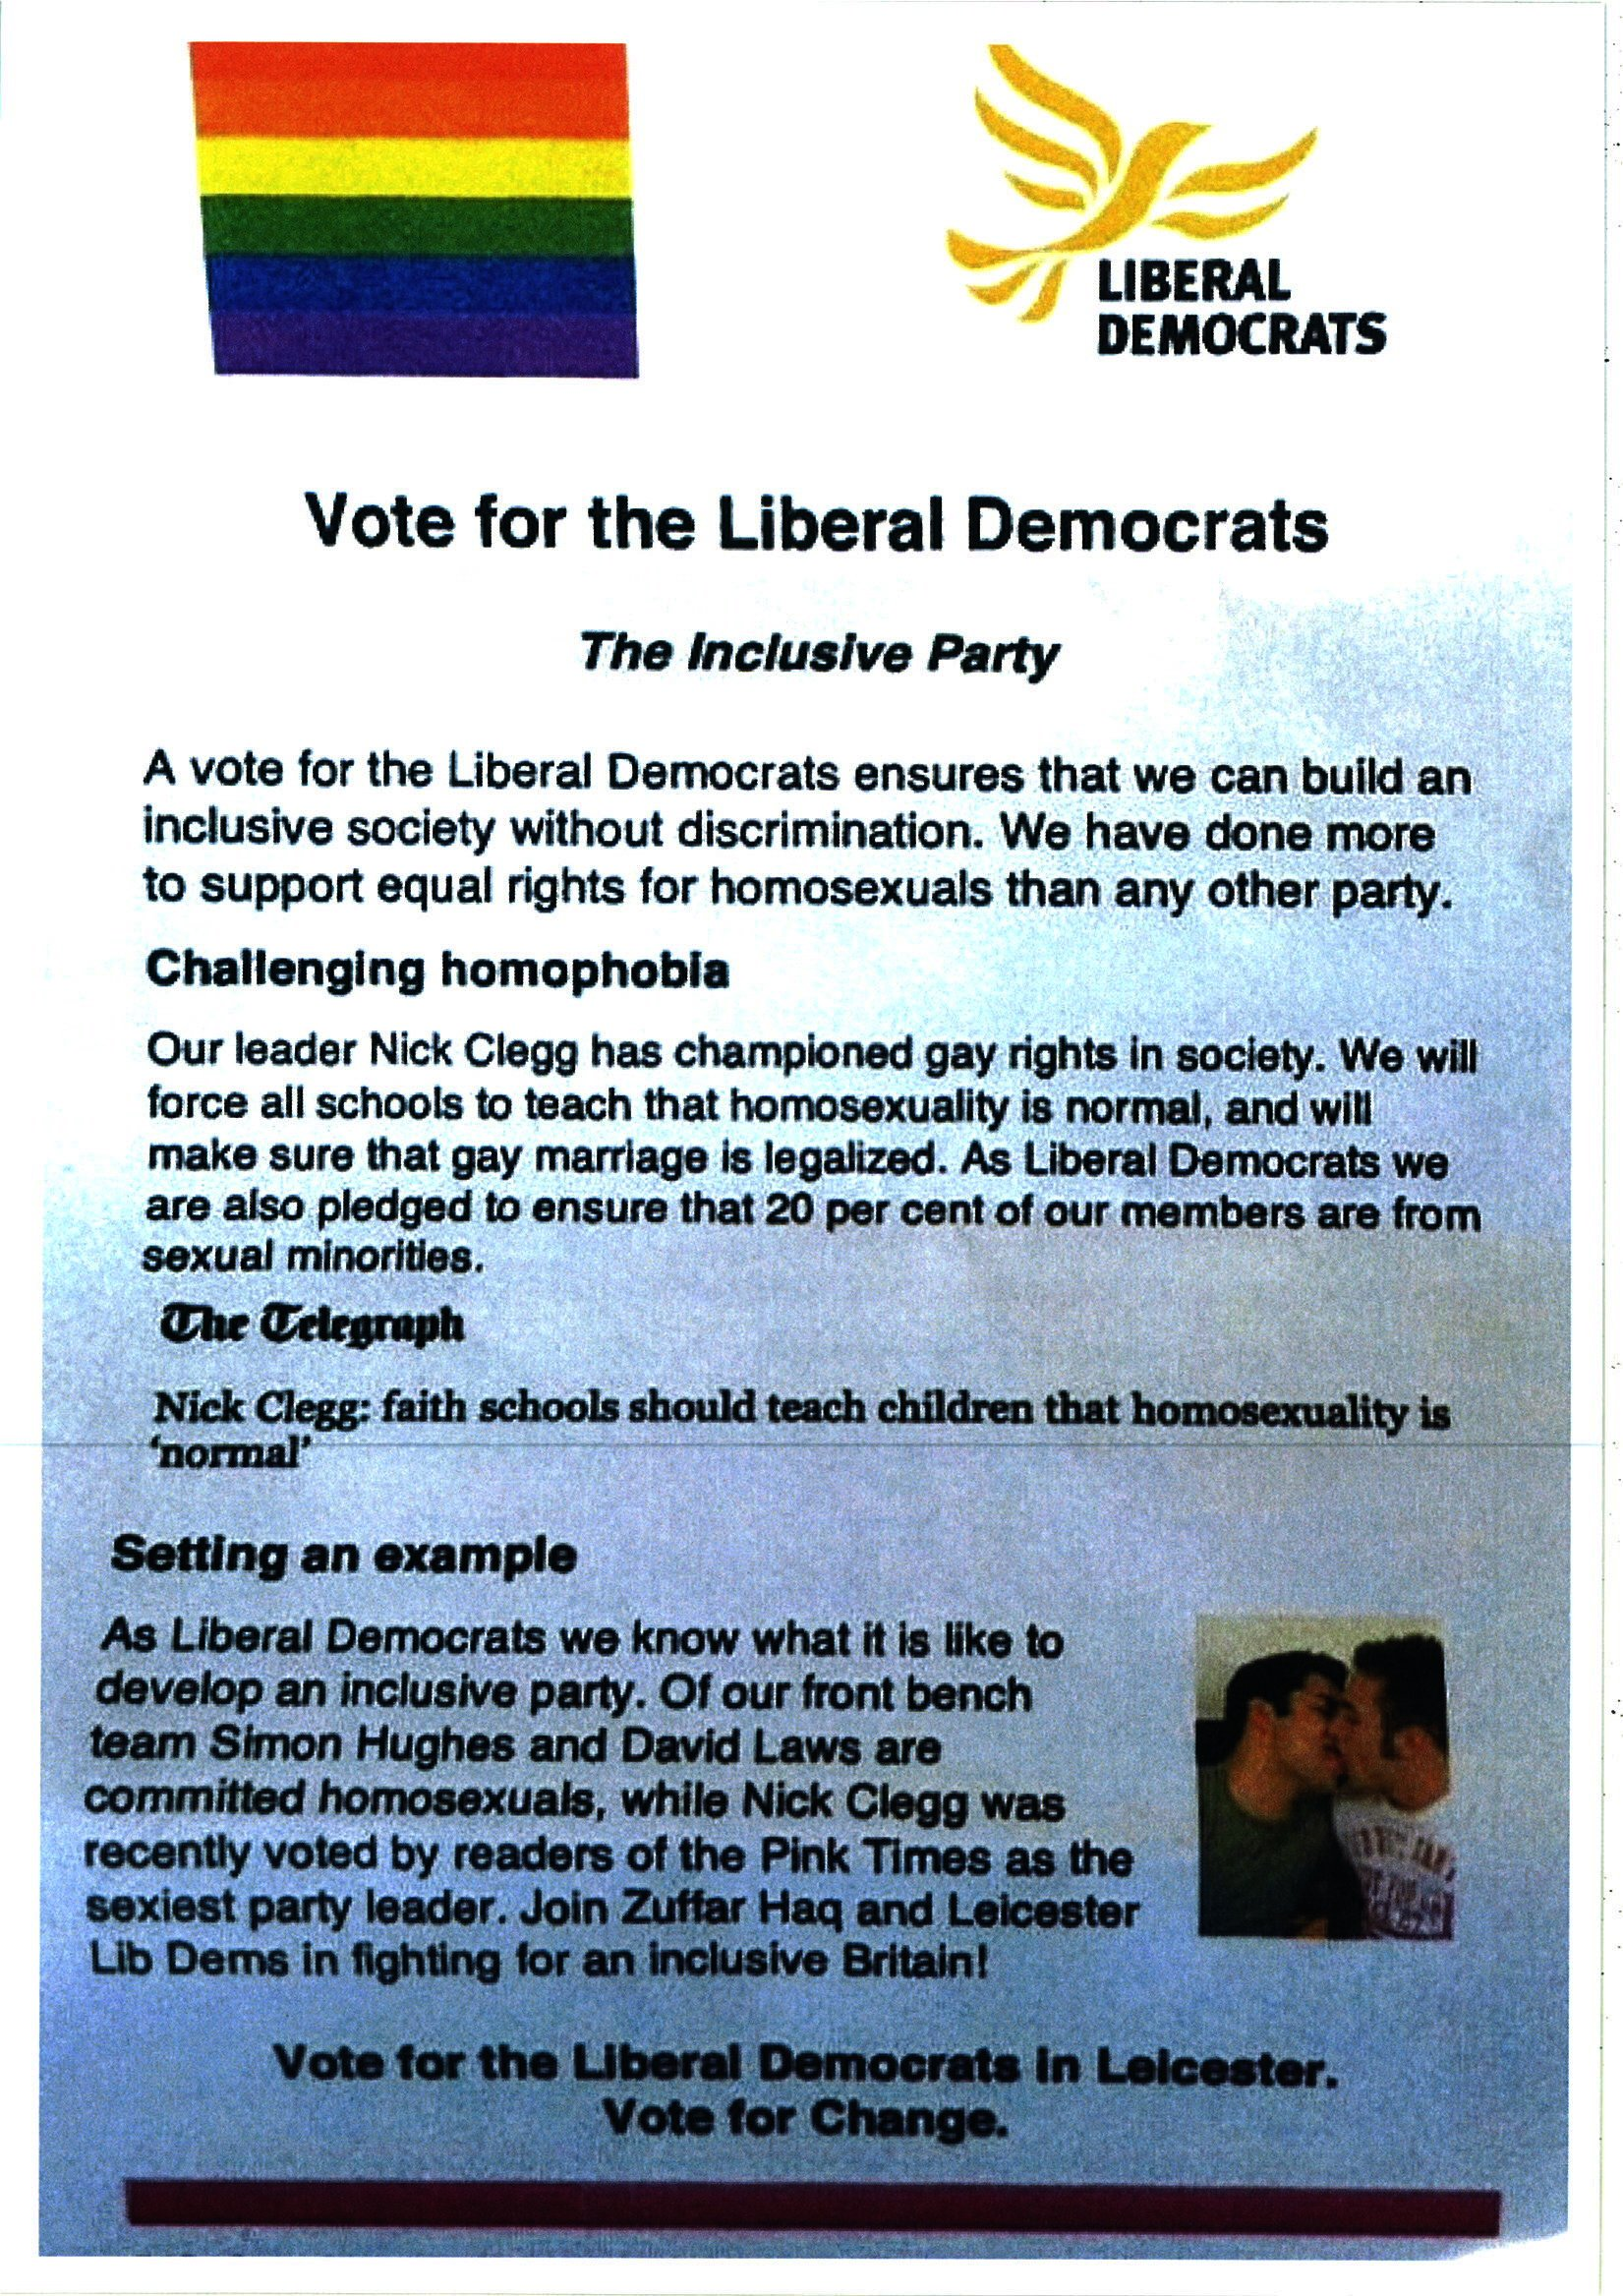
\includegraphics[scale=0.4]{images/FJEZNU.jpg}
		\caption{Image à traiter par OCRopus}
		\label{fig:image}
	\end{figure}

	\begin{figure}[H]
		\centering
		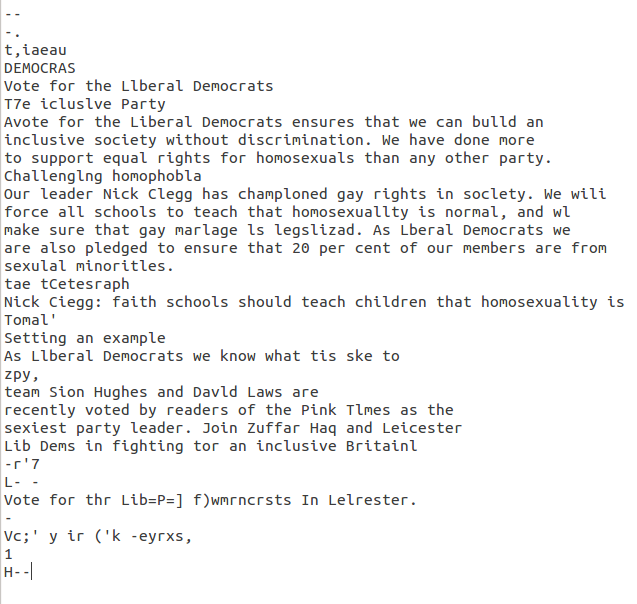
\includegraphics[scale=0.6]{images/FJEZNU_result.png}
		\caption{Texte trouvé par OCRopus}
		\label{fig:resultat}
	\end{figure}

	Avec cette image, on remarque que les lettre se ressemblant (i et l) sont souvent confondues, et que la qualité de l'image est importante : le bas de la page, moins bien éclairé, est mal reconnu et le mot "normal", situé sur la pliure, est interprété comme Tomal'. On remarque également que la police est importante : The Telegraph est interprété comme tae tCetesraph.

	Des essais sur d'autres images nous ont montré que la rotation est importante (une image tournée à 90 $\deg$ n'est pas du tout reconnue par OCRopus) ainsi que l'espacement entre les caractères, qui peut rendre la police plus ou moins "lisible". Enfin, les écritures manuscrites ne sont pas du tout reconnues pas OCRopus.

